\documentclass[a4paper, 12pt]{article}

\usepackage[polish]{babel}
\usepackage[a4paper,top=2cm,bottom=2cm,left=3cm,right=3cm,marginparwidth=1.75cm]{geometry}

\usepackage{listings}
\usepackage{polski}
\usepackage[utf8]{inputenc}
\usepackage{color}
\usepackage{setspace}
\usepackage{acro}
\usepackage{amsmath}
\usepackage{amsthm}
\usepackage[nottoc,numbib]{tocbibind}
\usepackage{graphicx}
\usepackage[table,xcdraw]{xcolor}
\usepackage{geometry}
\usepackage{subcaption}
\usepackage{movie15}
\usepackage{fancyvrb}
\usepackage{cancel}
\usepackage{tikz}
\usepackage{setspace}
\usepackage{color}
\documentclass{article}
\usepackage[utf8]{inputenc}
\usepackage{tikz}
\usetikzlibrary{positioning}
\usetikzlibrary{shapes,arrows,arrows,positioning,fit}
\usetikzlibrary{calc,trees,positioning,arrows,chains,shapes.geometric,%
    decorations.pathreplacing,decorations.pathmorphing,shapes,%
    matrix,shapes.symbols}
\include{acronyms}
\usepackage[colorlinks=true, allcolors=blue]{hyperref}
\definecolor{Code}{rgb}{0,0,0}
\definecolor{Decorators}{rgb}{0.5,0.5,0.5}
\definecolor{Numbers}{rgb}{0.5,0,0}
\definecolor{MatchingBrackets}{rgb}{0.25,0.5,0.5}
\definecolor{Keywords}{rgb}{0,0,1}
\definecolor{self}{rgb}{0,0,0}
\definecolor{Strings}{rgb}{0,0.63,0}
\definecolor{Comments}{rgb}{0,0.63,1}
\definecolor{Backquotes}{rgb}{0,0,0}
\definecolor{Classname}{rgb}{0,0,0}
\definecolor{FunctionName}{rgb}{0,0,.7}
\definecolor{Operators}{rgb}{0,0,0}
\definecolor{Background}{rgb}{0.98,0.98,0.98}

\lstdefinestyle{python}{
  numbers=left,
  numberstyle=\footnotesize,
  numbersep=1em,
  xleftmargin=1em,
  framextopmargin=1em,
  framexbottommargin=2em,
  showspaces=false,
  showtabs=false,
  showstringspaces=false,
  frame=l,
  tabsize=4,
  % Basic
  basicstyle=\ttfamily\small\setstretch{1},
  backgroundcolor=\color{Background},
  language=Python,
  % Comments
  commentstyle=\color{Comments}\slshape,
  % Strings
  stringstyle=\color{Strings},
  morecomment=[s][\color{Strings}]{"""}{"""},
  morecomment=[s][\color{Strings}]{'''}{'''},
  % keywords
  morekeywords={import,from,class,def,for,while,if,is,in,elif,else,not,and,or,print,break,continue,return,True,False,None,access,as,,del,except,exec,finally,global,import,lambda,pass,print,raise,try,assert},
  keywordstyle={\color{Keywords}\bfseries},
  % additional keywords
  morekeywords={[2]@invariant},
  keywordstyle={[2]\color{Decorators}\slshape},
  emph={self},
  emphstyle={\color{self}\slshape},
  breaklines=true
}
\title{Python - losowe zagadnienia}
\newline
\author{Kamil Musikowski}
\setstretch{1.50}
\begin{document}
\maketitle
\\
\begin{abstract}
   Projekt na zaliczenie warsztatu programisty.
   Wybrałem temat Python - losowe zagadnienia, dlatego iż że nie chciałem przepisywać gotowej książki, ani tutorialu pythona, co ktoś już pewnie zrobił.
\end{abstract}
\\ \\ \\
\tableofcontents

\pagebreak


\section{Mrówka langtona}

Jest to automat komórkowy jak i również \href{https://pl.wikipedia.org/wiki/Maszyna_Turinga}{Maszyna Turinga} działająca na następujących zasadach:
\begin{itemize}
    \item Na mapie składającej się z pełnych i pustych komórek pojawia się mrówka
    \item Jeśli mrówka znajduje się na polu pustym, to obraca się w lewo o 90\textdegree, po czym przechodzi na następną komórkę
    \item Jeśli znajdzie się na polu pełnym, obraca się w prawo o 90\textdegree i przechodzi na następną komórkę
\end{itemize}

\hfill 

Schemat blokowy: 
\hfill \hfill \break \hfill \hfill \break \hfill 
\begin{normalsize}
\tikzstyle{decision} = [diamond, draw, fill=blue!20, 
    text width=4.5em, text badly centered, node distance=5cm, inner sep=0pt]
\tikzstyle{block} = [rectangle, draw, fill=blue!20, 
    text width=5em, text centered, rounded corners, node distance=5cm, minimum height=4em]
\tikzstyle{line} = [draw, -latex']
\tikzstyle{cloud} = [draw, ellipse,fill=red!20, node distance=4cm,
    minimum height=2em]
    
\begin{tikzpicture}[node distance = 4cm, auto]
\node [cloud] (start) {start};
\node [decision, below of=start] (state) {sprawdź stan aktualnej komórki};
\node [block, left of=state] (pelna) {Obrót o 90\textdegree w prawo, zmień stan komórki na pusty};
\node [block, right of=state] (pusta) {Obrót o 90\textdegree w lewo, zmień stan komórki na pełny};
\node [block, below of=state] (ruch) {Przejdź na komórkę przed siebie};

\path [line] (start) -- (state);
\path [line] (state) -- node {k. pełna}(pelna);
\path [line] (state) -- node {k. pusta}(pusta);
\path [line] (pelna) |- node [near start] { } (ruch);
\path [line] (pusta) |- node [near start] { } (ruch);
\path [line] (ruch) -- (state);

\end{tikzpicture}
\end{normalsize}




\noindent\begin{minipage}{\linewidth}
\begin{lstlisting}[style=python]
class Ant:
    def __init__(self, y, x, direction):
        self.y = y
        self.x = x
        self.direction = direction
        
    def create_area(self, size):
        return [['[ ]' for _ in range(size)] for _ in range(size)]
    def change_area(self):
        if area[self.y][self.x] == '[ ]':
            area[self.y][self.x] = '[#]' 
        else:
            area[self.y][self.x] = '[ ]'
            
    def change_location(self):
        if self.direction == 1:
            self.y -= 1
        elif self.direction == 2:
            self.x += 1
        elif self.direction == 3:
            self.y += 1
        elif self.direction == 4:
            self.x -= 1

    def choose_turn_angle(self):
        if area[self.y][self.x] == '[ ]':
            return True
        else:
            return False

    def right_turn(self):
        self.direction += 1
        if self.direction == 5:
            self.direction = 1
    def left_turn(self):
        self.direction -= 1
        if self.direction == 0:
            self.direction = 4

    def show_area(self):
        for row in area:
            print(" ".join(map(str, row)))  # analyze

ant = Ant(7, 7, 1)  #startowe y, x, kierunek
area = ant.create_area(15) #wielkosc mapy
for reloads in range(400): #ilosc ruchow
    ant.change_area()
    ant.change_location()
    if ant.choose_turn_angle():
        ant.right_turn()
    else:
        ant.left_turn()
ant.show_area()

\end{lstlisting}
\end{minipage}


\pagebreak
Oto jak owy program może wyglądać, na wypadek gdyby komuś nie chciało się 

go włączać: 


\href{https://upload.wikimedia.org/wikipedia/commons/0/09/LangtonsAntAnimated.gif}{Przykładowy gif dla pierwszych 200 kroków}


\href{https://upload.wikimedia.org/wikipedia/commons/a/a3/MulticolorLangtonsAnt.gif}{Bardziej zaawansowana wersja}
\newline

Przykładowy wynik po 11000 kroków\cite{ant}:


\includegraphics[width=0.5\textwidth]{LangtonsAnt.png}

\\ \\ \\ \\ \\ \\ \\





\section{Operacje na listach}

\subsection{Slicing}

\\ \\
Przykładowe użycia slicingu. \\
Slicing może być używany na pętlach i tuplach.

\\
\noindent\begin{minipage}{\linewidth}
\begin{lstlisting}[style=python]
>>> numbers = [1, 2, 3, 4, 5, 6, 7, 8, 9]
>>> pierwsze_piec = numbers[0:5]
>>> pierwsze_piec[2] = 30
>>> pierwsze_piec
[1, 2, 30, 4, 5]
>>> numbers
[1, 2, 3, 4, 5, 6, 7, 8, 9]
\end{lstlisting}
\end{minipage}
\\ \\ 
\pagebreak

Wybieranie środkowych elementów listy:
\\

\noindent\begin{minipage}{\linewidth}
\begin{lstlisting}[style=python]
>>> numbers = [10, 20, 30, 40, 50, 60, 70, 80, 90]
>>> numbers[1:-1]
[20, 30, 40, 50, 60, 70, 80]
>>> numbers[-3:8]
[70, 80]
>>> numbers[-5:-1]
[50, 60, 70, 80]
\end{lstlisting}
\end{minipage}
\\ \\ \\
Przypisywanie wartości zmiennym za pomocą slicingu:
\\
\noindent\begin{minipage}{\linewidth}
\begin{lstlisting}[style=python]
>>> numbers = [10, 20, 30, 40, 50, 60, 70, 80, 90]
>>> numbers[:4] = [1,2,3,4]
>>> numbers
[1, 2, 3, 4, 50, 60, 70, 80, 90]
\end{lstlisting}
\end{minipage}
\\ \\ \\
Przypisywanie wartości i zmiana wielkości listy:
\\
\noindent\begin{minipage}{\linewidth}
\begin{lstlisting}[style=python]
>>> numbers = [10, 20, 30, 40, 50, 60, 70, 80, 90]
>>> numbers[:4] = [1,2,3,4,5,6,7]
>>> numbers
[1, 2, 3, 4, 5, 6, 7, 50, 60, 70, 80, 90]
\end{lstlisting}
\end{minipage}
\\ \\ \\
Zastępywanie co n-tego elementu:
\\
\noindent\begin{minipage}{\linewidth}
\begin{lstlisting}[style=python]
>>> numbers = [10, 20, 30, 40, 50, 60, 70, 80, 90]
>>> numbers[::2] = [1,1,1,1,1]
>>> numbers
[1, 20, 1, 40, 1, 60, 1, 80, 1]
\end{lstlisting}
\end{minipage}
\\ \\ \\
Zastępywanie co n-tego elementu, ale od końca:
\\
\noindent\begin{minipage}{\linewidth}
\begin{lstlisting}[style=python]
>>> numbers = [10, 20, 30, 40, 50, 60, 70, 80, 90]
>>> numbers[::-2] = [1,2,3,4,5]
>>> numbers
[5, 20, 4, 40, 3, 60, 2, 80, 1]
\end{lstlisting}
\end{minipage}
\\ \\ \\
Odwracanie listy:
\\
\noindent\begin{minipage}{\linewidth}
\begin{lstlisting}[style=python]
>>> numbers = [1, 2, 3, 4, 5, 6, 7, 8, 9]
>>> numbers[::-1]
[9, 8, 7, 6, 5, 4, 3, 2, 1]
\end{lstlisting}
\end{minipage}

\section{Przydatne funkcje}

\subsection{Funkcja lambda:}

Funkcję Lambda, inaczej można nazwać funkcją anonimową lub literałem 
\\
funkcyjnym.
Funkcja ta nie jest czymś, czego nie można osiągnąć za pomocą standardowych sposobów. Używa jej się przede wszystkim ze względu na wygodę i czytelność. Jest często używana raz, lub niewielką ilość razy, jest szczególnie przydatna w dziedzinie analizy danych, chociażby jako pomoc przy użyciu funkcji map(), filter(), reduce().
\\ \\
Użycie funkcji lambda wygląda następująco:

\noindent\begin{minipage}{\linewidth}
\begin{lstlisting}[style=python]
multiply = lambda x, y: x*y
multiply(3, 5)
\end{lstlisting}
\end{minipage}
\\ \\
I jest równoznaczne z:


\noindent\begin{minipage}{\linewidth}
\begin{lstlisting}[style=python]
def multiply(x, y):
    return x*y
    
multiply(3, 5)
\end{lstlisting}
\end{minipage}
\\ \\ \\
Przykładowe wywołanie i zwrócenie wartości z funkcji lambda, w inny sposób, bez przypisywania do zmiennej:

\noindent\begin{minipage}{\linewidth}
\begin{lstlisting}[style=python]
print((lambda x,y: (x*y)**2)(3,4))
\end{lstlisting}
\end{minipage}
\\
Output:


\noindent\begin{minipage}{\linewidth}
\begin{lstlisting}[style=python]
144
\end{lstlisting}
\end{minipage}
\\ \\ 

Losowa tabelka, ponieważ nie było okazji do jej użycia
\begin{table}[!ht]
    \centering
    \begin{tabular}{|l|l|l|l|}
    \hline
        \textbf{X} & \textbf{2} & \textbf{3} & \textbf{4} \\ \hline
        \textbf{5} & 10 & 15 & 20 \\ \hline
        \textbf{15} & 30 & 45 & 60 \\ \hline
        \textbf{50} & 100 & 150 & 200 \\ \hline
    \end{tabular}
\end{table}




\pagebreak

\subsection{Funkcja map()}
Funkcja map() pozwala na użycie danej funkcji dla każdego elementu iterowalnej struktury danych (np. listę lub krotkę).


Przykładowe użycia funkcji map():

\noindent\begin{minipage}{\linewidth}
\begin{lstlisting}[style=python]
def square(x):
    return x*x
    
numbers = [1, 2, 3, 4, 5, 6, 7, 8, 9]

answer = map(square, numbers)
print(answer)

numbersSquare = list(result)
print(numbersSquare)
\end{lstlisting}
\end{minipage}
\\ \\
Output:


\noindent\begin{minipage}{\linewidth}
\begin{lstlisting}[style=python]
<map object at 0x000002E3FFED8C10>
[1, 4, 9, 16, 25, 36, 49, 64, 81]
\end{lstlisting}
\end{minipage}
\\ \\
Jak widać, przed wywołaniem wartości zwracanej przez map(), musimy przekonwertować ją na odpowiednią strukturę, np. list(), tuple() lub set().
\\ \\ \\
Kwadrat liczb w liście za pomocą połączenia funkcji map() i Lambda:

\noindent\begin{minipage}{\linewidth}
\begin{lstlisting}[style=python]
numbers = (1, 2, 3, 4, 5, 6)
answer = map(lambda x: x**x, numbers)
print(list(answer))
\end{lstlisting}
\end{minipage}
\\ \\ \\
Możemy także operować na wielu strukturach:

\noindent\begin{minipage}{\linewidth}
\begin{lstlisting}[style=python]
num1 = [1, 2, 3]
num2 = [5, 6, 7]
num3 = [10, 20, 30]

answer = map(lambda x, y, z: x + y + z, num1, num2, num3)
print(list(answer))
\end{lstlisting}
\end{minipage}

\pagebreak

\subsection{Funkcja filter()}
Funkcja filter() zwraca elementy iteralnej struktury, dla których wartość wynosi True dla danej funkcji.
\\ \\
Przykładowe użycia funkcji:
\\ \\
\noindent\begin{minipage}{\linewidth}
\begin{lstlisting}[style=python]
numbers = [1, 2, 3, 4, 5, 6, 7, 8, 9]

def even(number):
    if number % 2 == 0:
          return True
    return False

print(tuple(filter(even, numbers)))
\end{lstlisting}
\end{minipage}
\\ \\ 
Output:


\noindent\begin{minipage}{\linewidth}
\begin{lstlisting}[style=python]
(2, 4, 6, 8)
\end{lstlisting}
\end{minipage}
\\ \\
Zwracanie liczb podzielnych przez 11 przy pomocy funkcji Lambda:


\noindent\begin{minipage}{\linewidth}
\begin{lstlisting}[style=python]
numbers = list(range(100))

answer = filter(lambda x: x % 11 == 0, numbers)

print(list(answer))
\end{lstlisting}
\end{minipage}
\\ \\
Output:

\noindent\begin{minipage}{\linewidth}
\begin{lstlisting}[style=python]
[0, 11, 22, 33, 44, 55, 66, 77, 88, 99]
\end{lstlisting}
\end{minipage}
\\ \\ 
Możemy też operować na literach:


\noindent\begin{minipage}{\linewidth}
\begin{lstlisting}[style=python]
letters = ['a', 'p', 'd', 'x', 'i', 'j', 'e', 'z', 's']

def check_word(letter):
    search = ['p', 'e', 'i', 'o', 'e', 's']
    return True if letter in search else False

word = filter(check_word, letters)

print(list(word))
\end{lstlisting}
\end{minipage}
\\ \\
Output:

\noindent\begin{minipage}{\linewidth}
\begin{lstlisting}[style=python]
['p', 'i', 'e', 's']
\end{lstlisting}
\end{minipage}
\pagebreak

\section{Inne przydatne rzeczy}

\subsection{f-strings}
f-stringsy umożliwiają o wiele wygodniejsze i krótsze zapisywanie tekstu w  \\ funkcji printf() 

\noindent\begin{minipage}{\linewidth}
\begin{lstlisting}[style=python]
>>> a = 10
>>> b = "<"
>>> f"a wynosi {a} i jest {b} od 100"
>>> a wynosi 10 i jest < od 100
\end{lstlisting}
\end{minipage}
\\ \\

\subsection{Walrus operator}
Walrus operator, opisywany za pomocą znaków ":=" jest nową funkcjonalnością i został dodany w Pythonie 3.8.
Pozwala na nadanie wartości zmiennej w obrębie danego wyrażenia.


\noindent\begin{minipage}{\linewidth}
\begin{lstlisting}[style=python]
a = 10
if (x := a) > 3:
    print(f"{x} jest > 3")
\end{lstlisting}
\end{minipage}
\\ \\
Operator może być użyteczny podczas pętli\cite{wal}:


\noindent\begin{minipage}{\linewidth}
\begin{lstlisting}[style=python]
sample_data = [
    {"userId": 1, "name": "rahul", "completed": False},
    {"userId": 1, "name": "rohit", "completed": False},
    {"userId": 1, "name": "ram", "completed": False},
    {"userId": 1, "name": "ravan", "completed": True}
]

print("With Python 3.8 Walrus Operator:")
for entry in sample_data:
    if name := entry.get("name"):
        print(f'Found name: "{name}"')

print("Without Walrus operator:")
for entry in sample_data:
    name = entry.get("name")
    if name:
        print(f'Found name: "{name}"')
\end{lstlisting}
\end{minipage}
\pagebreak

\section{Popularność}
Popularność pythona na tle innych języków według \\
Stack Overflow Developer Survey 2021\cite{stack}
\\
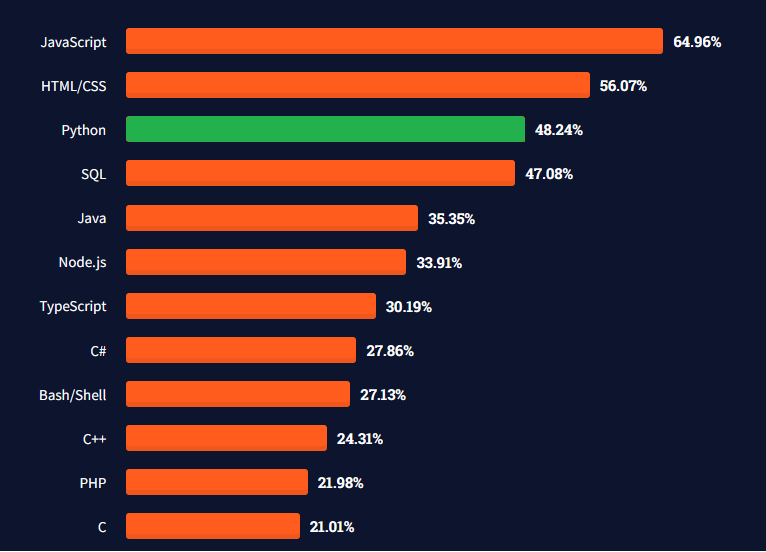
\includegraphics[width=1.1\textwidth]{stack.png}
\\ \\
Popularność frameworków pythona według ankiety bulldogjob 2021\cite{bull}\\
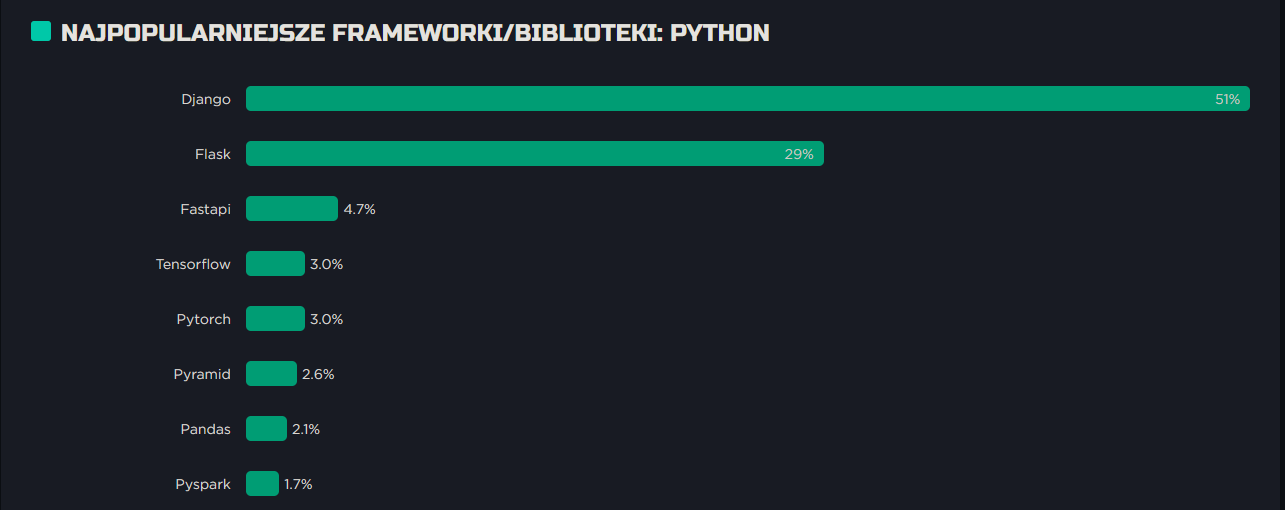
\includegraphics[width=1.1\textwidth]{bull.png}


\pagebreak


\begin{thebibliography}{9}
\bibitem{stack}
\href{https://insights.stackoverflow.com/survey/2021#most-popular-technologies-language}{https://insights.stackoverflow.com/survey/2021#most-popular-technologies-language} 

\bibitem{bull}
\href{https://bulldogjob.pl/it-report/2021/programmer}{https://bulldogjob.pl/it-report/2021/programmer} 


\bibitem{wal}
\href{https://www.geeksforgeeks.org/walrus-operator-in-python-3-8/}{https://www.geeksforgeeks.org/walrus-operator-in-python-3-8/}

\bibitem{ant}
\href{https://en.wikipedia.org/wiki/Langtons_ant}{https://en.wikipedia.org/wiki/Langtons_ant}

\end{thebibliography}
\end{document}